\section{Results}
\label{sec:results}

FFTT-like setup with a total collecting area of $(\Delta L)^2$=4 km$^2$, $\Omega_\text{survey}=1$sr, $t_\text{obs}$=1 year, assuming the array observed redshifts in the range $z\in [10,35]$. Figure \ref{fig:B0zeta_vs_deltas} shows how this sensitivity changes as a function of the maximum baseline.
\begin{figure}
\centering
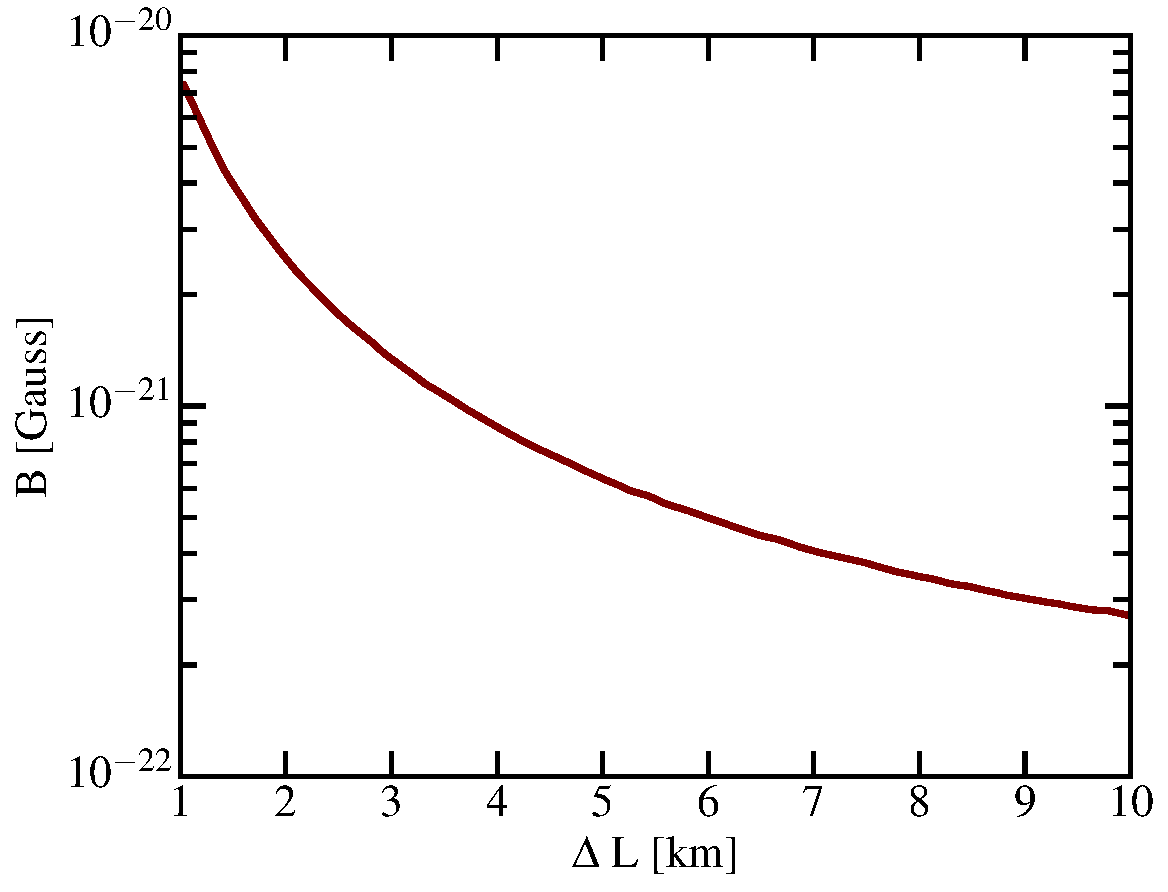
\includegraphics[width=.35\textwidth,keepaspectratio=true]{B0_vs_deltas.pdf}
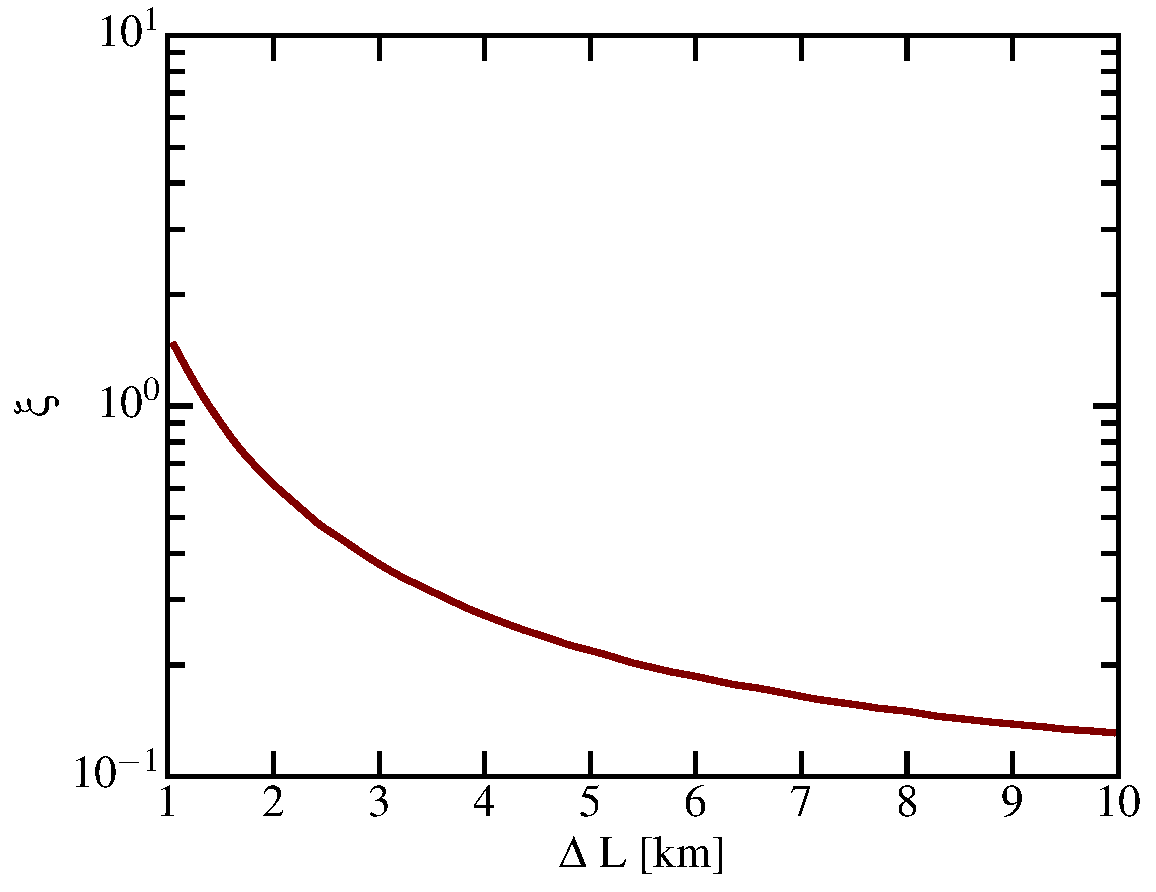
\includegraphics[width=.35\textwidth,keepaspectratio=true]{zeta_vs_deltas.pdf}
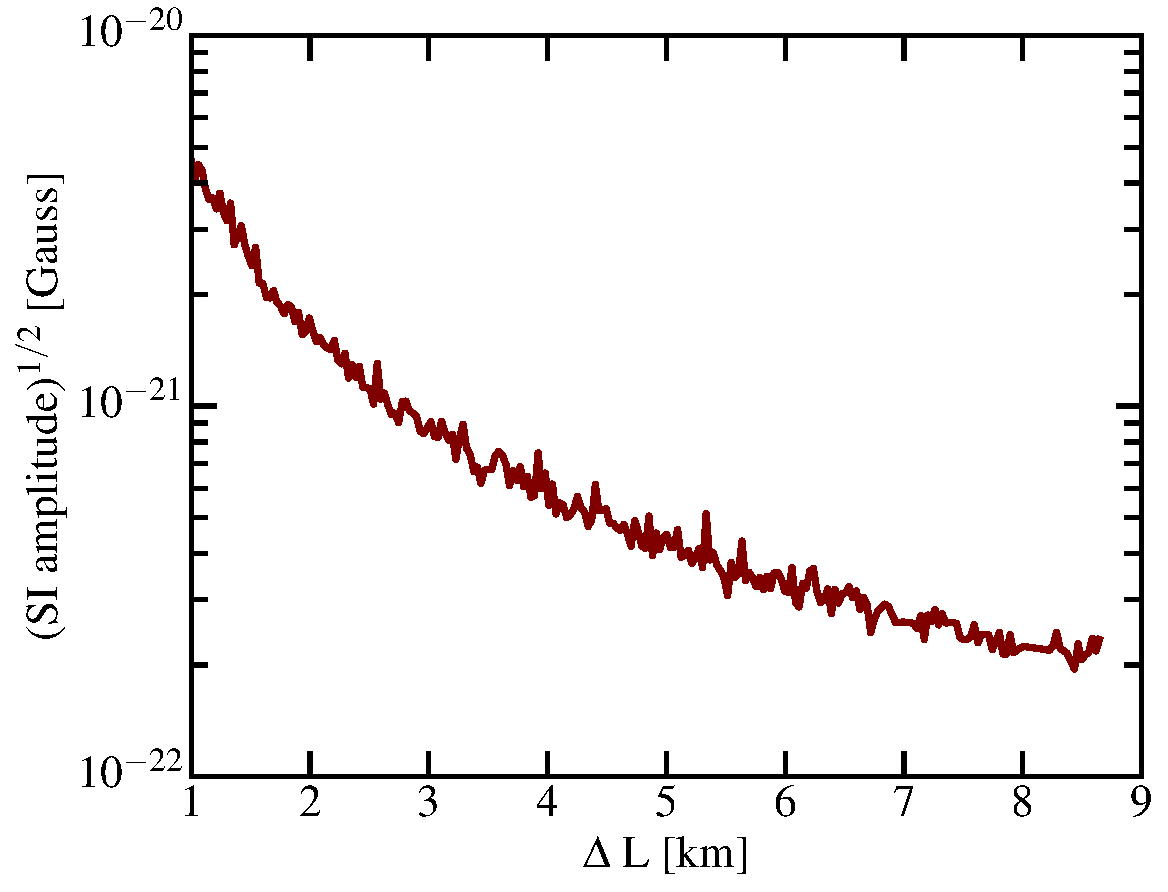
\includegraphics[width=.35\textwidth,keepaspectratio=true]{SI_vs_deltas.pdf}
\caption{FFTT sensitivity to detecting a uniform magnetic field (left panel), and to distinguishing saturated case from no magnetic field (right panel), as a function of maximum baseline. Both are calculated for a survey size of 1 sr, assuming a uniform magnetic field in the entire survey volume.\label{fig:B0zetaSI_vs_deltas}}
\end{figure}
\begin{figure}
\centering
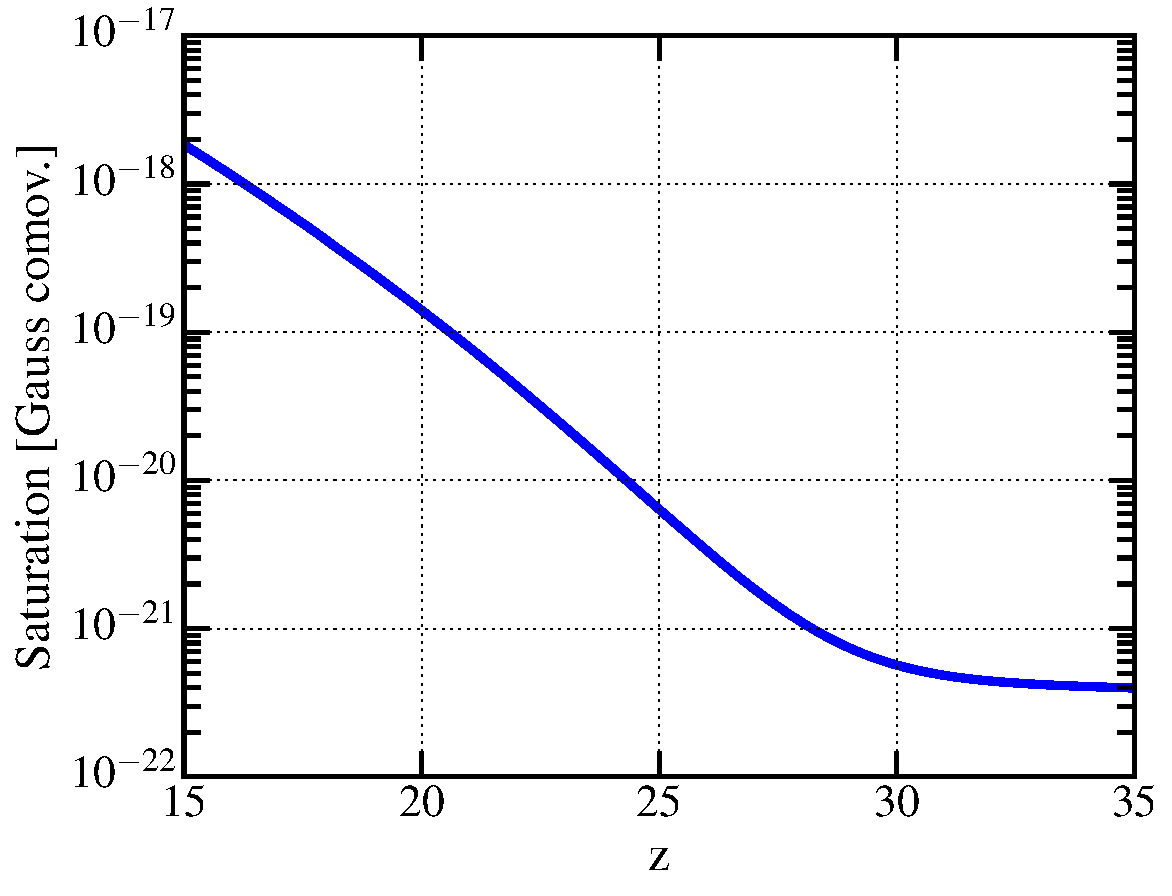
\includegraphics[width=.35\textwidth,keepaspectratio=true]{Bsaturation.pdf}
\caption{FFTT.\label{fig:Bsat}}
\end{figure}